\documentclass[11pt,a4paper,]{article}
\usepackage{lmodern}

\usepackage{amssymb,amsmath}
\usepackage{ifxetex,ifluatex}
\usepackage{fixltx2e} % provides \textsubscript
\ifnum 0\ifxetex 1\fi\ifluatex 1\fi=0 % if pdftex
  \usepackage[T1]{fontenc}
  \usepackage[utf8]{inputenc}
\else % if luatex or xelatex
  \usepackage{unicode-math}
  \defaultfontfeatures{Ligatures=TeX,Scale=MatchLowercase}
\fi
% use upquote if available, for straight quotes in verbatim environments
\IfFileExists{upquote.sty}{\usepackage{upquote}}{}
% use microtype if available
\IfFileExists{microtype.sty}{%
\usepackage[]{microtype}
\UseMicrotypeSet[protrusion]{basicmath} % disable protrusion for tt fonts
}{}
\PassOptionsToPackage{hyphens}{url} % url is loaded by hyperref
\usepackage[unicode=true]{hyperref}
\hypersetup{
            pdftitle={Analysis on Japan\&United State},
            pdfborder={0 0 0},
            breaklinks=true}
\urlstyle{same}  % don't use monospace font for urls
\usepackage{geometry}
\geometry{a4paper, centering, text={16cm,24cm}}
\usepackage[style=authoryear-comp,]{biblatex}
\addbibresource{references.bib}
\usepackage{color}
\usepackage{fancyvrb}
\newcommand{\VerbBar}{|}
\newcommand{\VERB}{\Verb[commandchars=\\\{\}]}
\DefineVerbatimEnvironment{Highlighting}{Verbatim}{commandchars=\\\{\}}
% Add ',fontsize=\small' for more characters per line
\usepackage{framed}
\definecolor{shadecolor}{RGB}{248,248,248}
\newenvironment{Shaded}{\begin{snugshade}}{\end{snugshade}}
\newcommand{\AlertTok}[1]{\textcolor[rgb]{0.94,0.16,0.16}{#1}}
\newcommand{\AnnotationTok}[1]{\textcolor[rgb]{0.56,0.35,0.01}{\textbf{\textit{#1}}}}
\newcommand{\AttributeTok}[1]{\textcolor[rgb]{0.77,0.63,0.00}{#1}}
\newcommand{\BaseNTok}[1]{\textcolor[rgb]{0.00,0.00,0.81}{#1}}
\newcommand{\BuiltInTok}[1]{#1}
\newcommand{\CharTok}[1]{\textcolor[rgb]{0.31,0.60,0.02}{#1}}
\newcommand{\CommentTok}[1]{\textcolor[rgb]{0.56,0.35,0.01}{\textit{#1}}}
\newcommand{\CommentVarTok}[1]{\textcolor[rgb]{0.56,0.35,0.01}{\textbf{\textit{#1}}}}
\newcommand{\ConstantTok}[1]{\textcolor[rgb]{0.00,0.00,0.00}{#1}}
\newcommand{\ControlFlowTok}[1]{\textcolor[rgb]{0.13,0.29,0.53}{\textbf{#1}}}
\newcommand{\DataTypeTok}[1]{\textcolor[rgb]{0.13,0.29,0.53}{#1}}
\newcommand{\DecValTok}[1]{\textcolor[rgb]{0.00,0.00,0.81}{#1}}
\newcommand{\DocumentationTok}[1]{\textcolor[rgb]{0.56,0.35,0.01}{\textbf{\textit{#1}}}}
\newcommand{\ErrorTok}[1]{\textcolor[rgb]{0.64,0.00,0.00}{\textbf{#1}}}
\newcommand{\ExtensionTok}[1]{#1}
\newcommand{\FloatTok}[1]{\textcolor[rgb]{0.00,0.00,0.81}{#1}}
\newcommand{\FunctionTok}[1]{\textcolor[rgb]{0.00,0.00,0.00}{#1}}
\newcommand{\ImportTok}[1]{#1}
\newcommand{\InformationTok}[1]{\textcolor[rgb]{0.56,0.35,0.01}{\textbf{\textit{#1}}}}
\newcommand{\KeywordTok}[1]{\textcolor[rgb]{0.13,0.29,0.53}{\textbf{#1}}}
\newcommand{\NormalTok}[1]{#1}
\newcommand{\OperatorTok}[1]{\textcolor[rgb]{0.81,0.36,0.00}{\textbf{#1}}}
\newcommand{\OtherTok}[1]{\textcolor[rgb]{0.56,0.35,0.01}{#1}}
\newcommand{\PreprocessorTok}[1]{\textcolor[rgb]{0.56,0.35,0.01}{\textit{#1}}}
\newcommand{\RegionMarkerTok}[1]{#1}
\newcommand{\SpecialCharTok}[1]{\textcolor[rgb]{0.00,0.00,0.00}{#1}}
\newcommand{\SpecialStringTok}[1]{\textcolor[rgb]{0.31,0.60,0.02}{#1}}
\newcommand{\StringTok}[1]{\textcolor[rgb]{0.31,0.60,0.02}{#1}}
\newcommand{\VariableTok}[1]{\textcolor[rgb]{0.00,0.00,0.00}{#1}}
\newcommand{\VerbatimStringTok}[1]{\textcolor[rgb]{0.31,0.60,0.02}{#1}}
\newcommand{\WarningTok}[1]{\textcolor[rgb]{0.56,0.35,0.01}{\textbf{\textit{#1}}}}
\usepackage{longtable,booktabs}
% Fix footnotes in tables (requires footnote package)
\IfFileExists{footnote.sty}{\usepackage{footnote}\makesavenoteenv{long table}}{}
\IfFileExists{parskip.sty}{%
\usepackage{parskip}
}{% else
\setlength{\parindent}{0pt}
\setlength{\parskip}{6pt plus 2pt minus 1pt}
}
\setlength{\emergencystretch}{3em}  % prevent overfull lines
\providecommand{\tightlist}{%
  \setlength{\itemsep}{0pt}\setlength{\parskip}{0pt}}
\setcounter{secnumdepth}{5}

% set default figure placement to htbp
\makeatletter
\def\fps@figure{htbp}
\makeatother


\title{Analysis on Japan\&United State}

%% MONASH STUFF

%% CAPTIONS
\RequirePackage{caption}
\DeclareCaptionStyle{italic}[justification=centering]
 {labelfont={bf},textfont={it},labelsep=colon}
\captionsetup[figure]{style=italic,format=hang,singlelinecheck=true}
\captionsetup[table]{style=italic,format=hang,singlelinecheck=true}


%% FONT
\RequirePackage{bera}
\RequirePackage[charter,expert,sfscaled]{mathdesign}
\RequirePackage{fontawesome}

%% HEADERS AND FOOTERS
\RequirePackage{fancyhdr}
\pagestyle{fancy}
\rfoot{\Large\sffamily\raisebox{-0.1cm}{\textbf{\thepage}}}
\makeatletter
\lhead{\textsf{\expandafter{\@title}}}
\makeatother
\rhead{}
\cfoot{}
\setlength{\headheight}{15pt}
\renewcommand{\headrulewidth}{0.4pt}
\renewcommand{\footrulewidth}{0.4pt}
\fancypagestyle{plain}{%
\fancyhf{} % clear all header and footer fields
\fancyfoot[C]{\sffamily\thepage} % except the center
\renewcommand{\headrulewidth}{0pt}
\renewcommand{\footrulewidth}{0pt}}

%% MATHS
\RequirePackage{bm,amsmath}
\allowdisplaybreaks

%% GRAPHICS
\RequirePackage{graphicx}
\setcounter{topnumber}{2}
\setcounter{bottomnumber}{2}
\setcounter{totalnumber}{4}
\renewcommand{\topfraction}{0.85}
\renewcommand{\bottomfraction}{0.85}
\renewcommand{\textfraction}{0.15}
\renewcommand{\floatpagefraction}{0.8}


%\RequirePackage[section]{placeins}

%% SECTION TITLES


%% SECTION TITLES (NEW: Changing sections and subsections color)
\RequirePackage[compact,sf,bf]{titlesec}
\titleformat*{\section}{\Large\sf\bfseries\color[rgb]{0.8, 0.7, 0.1 }}
\titleformat*{\subsection}{\large\sf\bfseries\color[rgb]{0.8, 0.7, 0.1 }}
\titleformat*{\subsubsection}{\sf\bfseries\color[rgb]{0.8, 0.7, 0.1 }}
\titlespacing{\section}{0pt}{2ex}{.5ex}
\titlespacing{\subsection}{0pt}{1.5ex}{0ex}
\titlespacing{\subsubsection}{0pt}{.5ex}{0ex}


%% TITLE PAGE
\def\Date{\number\day}
\def\Month{\ifcase\month\or
 January\or February\or March\or April\or May\or June\or
 July\or August\or September\or October\or November\or December\fi}
\def\Year{\number\year}

%% LINE AND PAGE BREAKING
\sloppy
\clubpenalty = 10000
\widowpenalty = 10000
\brokenpenalty = 10000
\RequirePackage{microtype}

%% PARAGRAPH BREAKS
\setlength{\parskip}{1.4ex}
\setlength{\parindent}{0em}

%% HYPERLINKS
\RequirePackage{xcolor} % Needed for links
\definecolor{darkblue}{rgb}{0,0,.6}
\RequirePackage{url}

\makeatletter
\@ifpackageloaded{hyperref}{}{\RequirePackage{hyperref}}
\makeatother
\hypersetup{
     citecolor=0 0 0,
     breaklinks=true,
     bookmarksopen=true,
     bookmarksnumbered=true,
     linkcolor=darkblue,
     urlcolor=blue,
     citecolor=darkblue,
     colorlinks=true}

\usepackage[showonlyrefs]{mathtools}
\usepackage[no-weekday]{eukdate}

%% BIBLIOGRAPHY

\makeatletter
\@ifpackageloaded{biblatex}{}{\usepackage[style=authoryear-comp, backend=biber, natbib=true]{biblatex}}
\makeatother
\ExecuteBibliographyOptions{bibencoding=utf8,minnames=1,maxnames=3, maxbibnames=99,dashed=false,terseinits=true,giveninits=true,uniquename=false,uniquelist=false,doi=false, isbn=false,url=true,sortcites=false}

\DeclareFieldFormat{url}{\texttt{\url{#1}}}
\DeclareFieldFormat[article]{pages}{#1}
\DeclareFieldFormat[inproceedings]{pages}{\lowercase{pp.}#1}
\DeclareFieldFormat[incollection]{pages}{\lowercase{pp.}#1}
\DeclareFieldFormat[article]{volume}{\mkbibbold{#1}}
\DeclareFieldFormat[article]{number}{\mkbibparens{#1}}
\DeclareFieldFormat[article]{title}{\MakeCapital{#1}}
\DeclareFieldFormat[article]{url}{}
%\DeclareFieldFormat[book]{url}{}
%\DeclareFieldFormat[inbook]{url}{}
%\DeclareFieldFormat[incollection]{url}{}
%\DeclareFieldFormat[inproceedings]{url}{}
\DeclareFieldFormat[inproceedings]{title}{#1}
\DeclareFieldFormat{shorthandwidth}{#1}
%\DeclareFieldFormat{extrayear}{}
% No dot before number of articles
\usepackage{xpatch}
\xpatchbibmacro{volume+number+eid}{\setunit*{\adddot}}{}{}{}
% Remove In: for an article.
\renewbibmacro{in:}{%
  \ifentrytype{article}{}{%
  \printtext{\bibstring{in}\intitlepunct}}}

\AtEveryBibitem{\clearfield{month}}
\AtEveryCitekey{\clearfield{month}}

\makeatletter
\DeclareDelimFormat[cbx@textcite]{nameyeardelim}{\addspace}
\makeatother

\author{\sf\Large\textbf{ Shu Wang}\\ {\sf\large Student\\[0.5cm]}}

\date{\sf\Date~\Month~\Year}
\makeatletter
\lfoot{\sf Wang: \@date}
\makeatother


%%%% PAGE STYLE FOR FRONT PAGE OF REPORTS

\makeatletter
\def\organization#1{\gdef\@organization{#1}}
\def\telephone#1{\gdef\@telephone{#1}}
\def\email#1{\gdef\@email{#1}}
\makeatother
  \organization{Australian Government COVID19}

  \def\name{Our consultancy \newline add names \&\newline add names}

  \telephone{(03) 9905 2478}

  \email{questions@company.com}                 %NEW: New email addresss

\def\webaddress{\url{http://company.com/stats/consulting/}} %NEW: URl
\def\abn{12 377 614 630}                                    % NEW: ABN
\def\logo{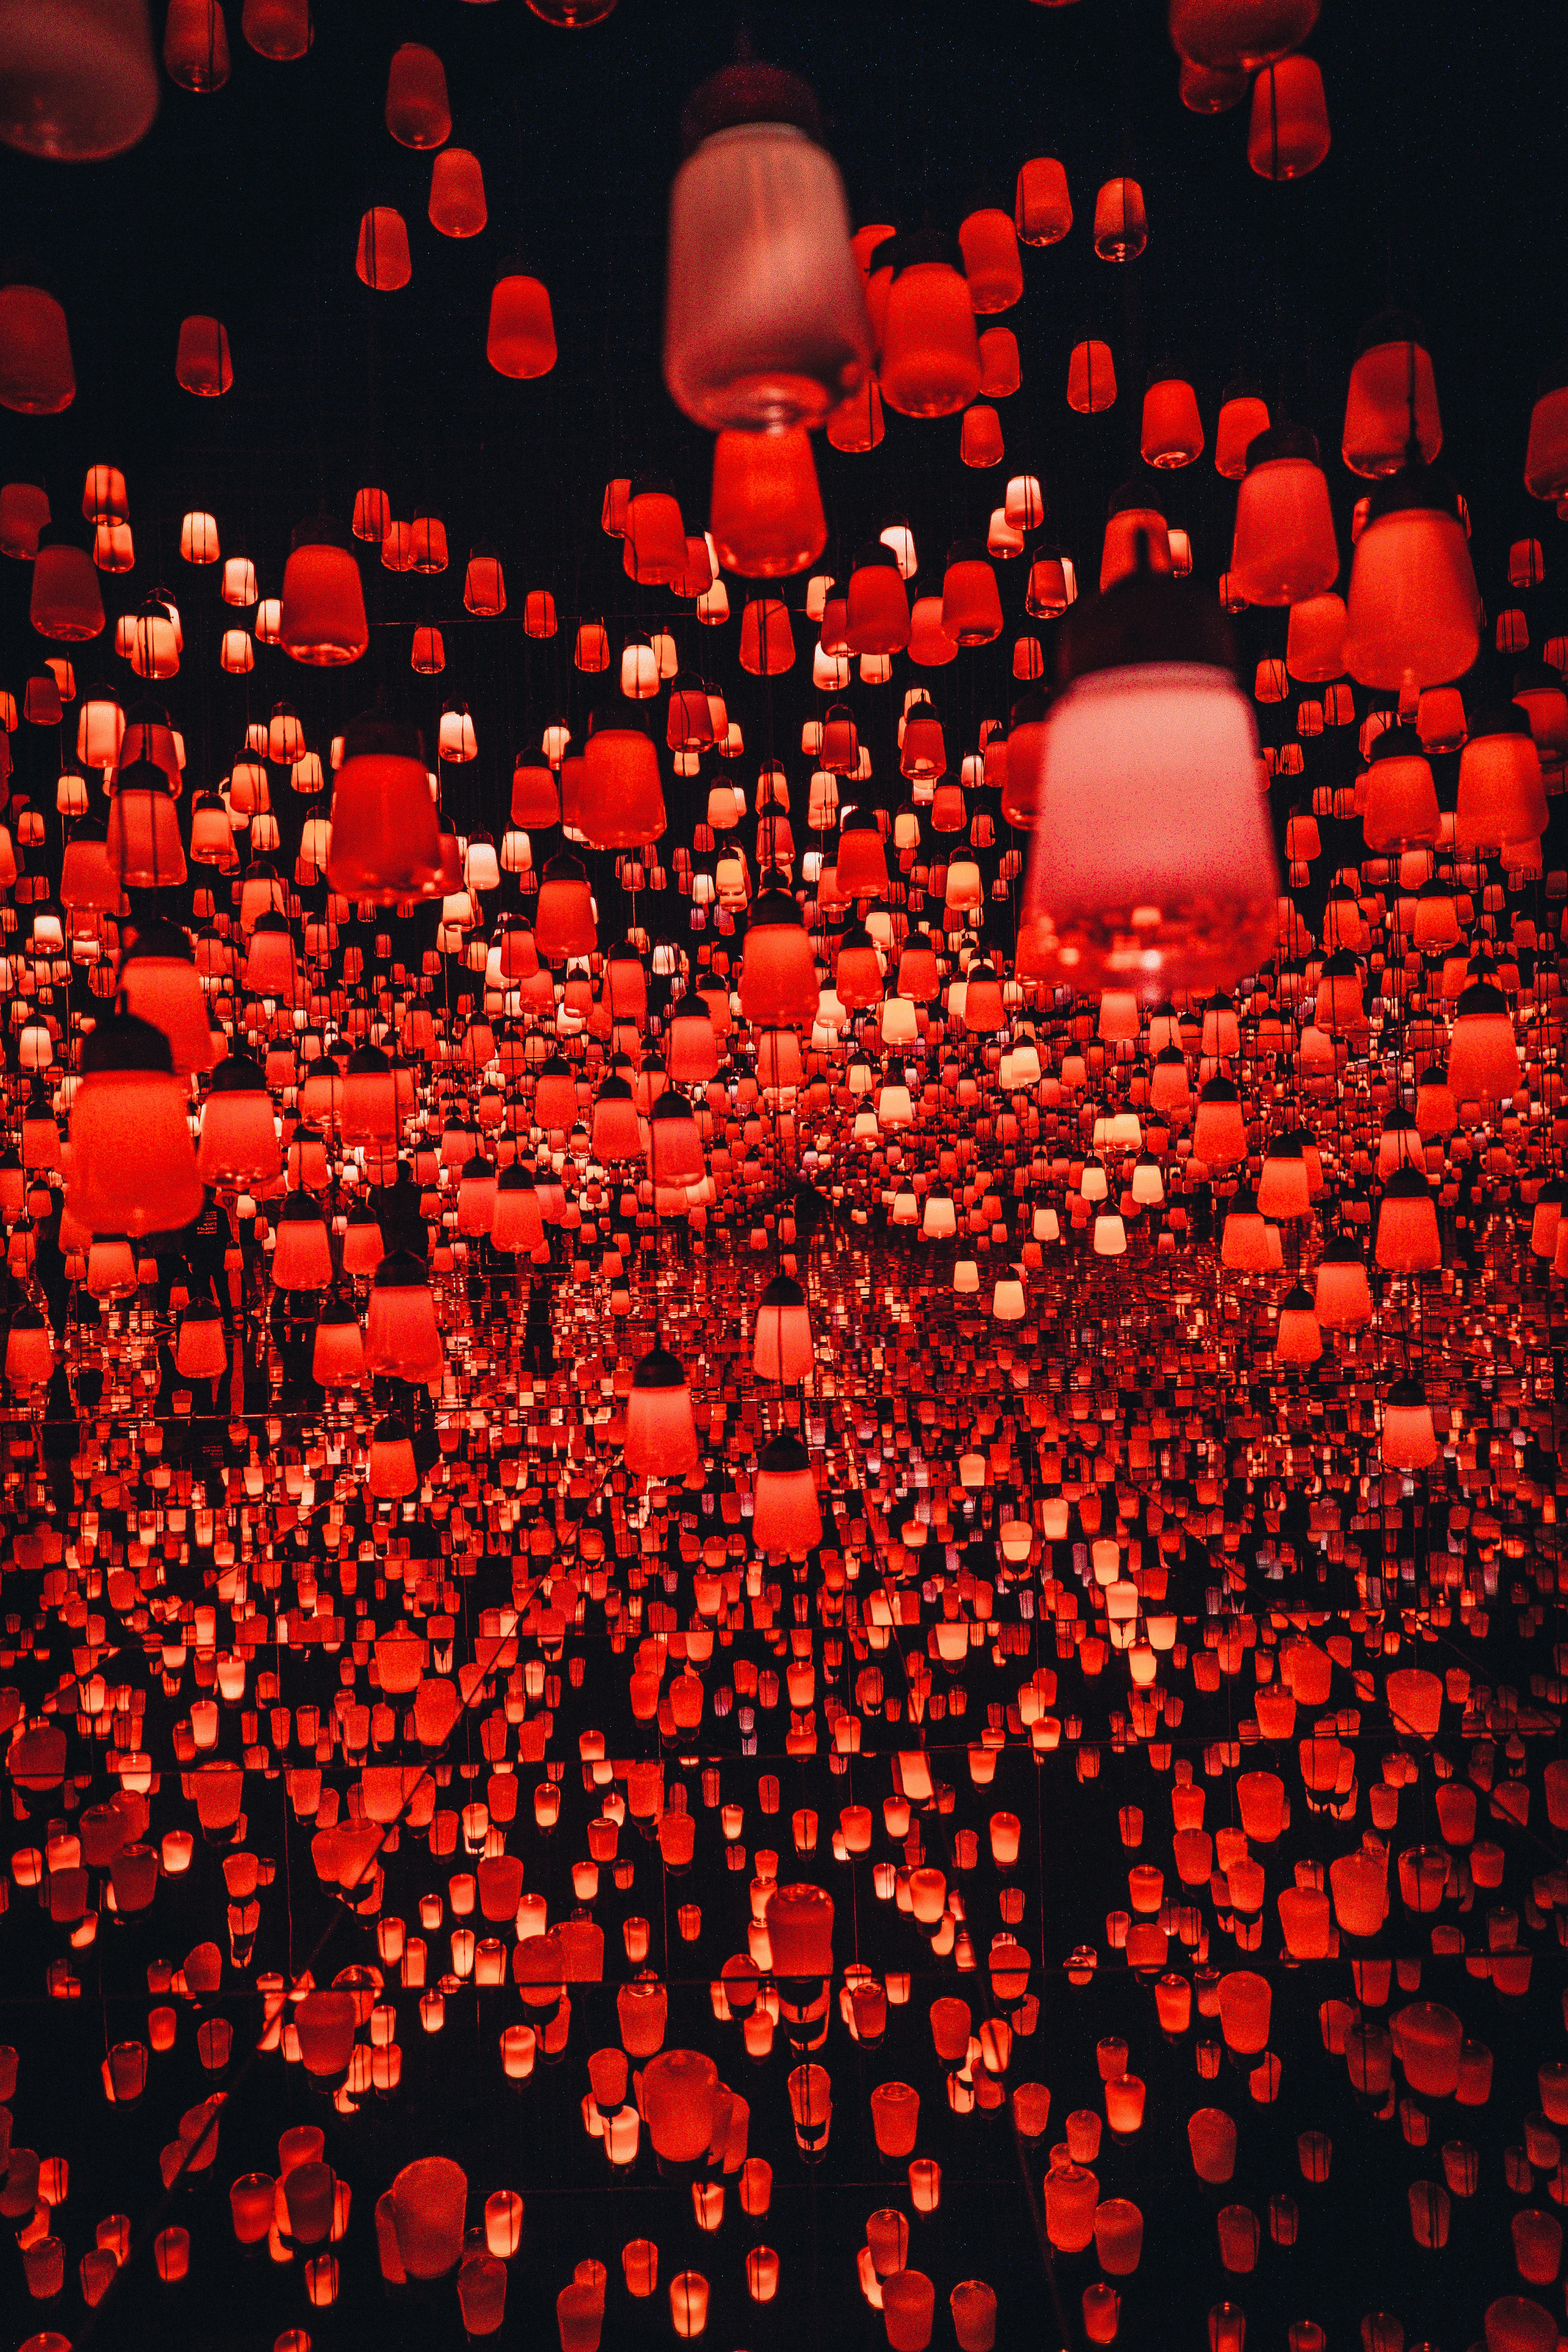
\includegraphics[width=6cm]{Figures/logo}}  %NEW: Changing logo
\def\extraspace{\vspace*{1.6cm}}
\makeatletter
\def\contactdetails{\faicon{phone} & \@telephone \\
                    \faicon{envelope} & \@email}
\makeatother

%%%% FRONT PAGE OF REPORTS

\def\reporttype{Report for}

\long\def\front#1#2#3{
\newpage
\begin{singlespacing}
\thispagestyle{empty}
\vspace*{-1.4cm}
\hspace*{-1.4cm}
\hbox to 16cm{
  \hbox to 6.5cm{\vbox to 14cm{\vbox to 25cm{
    \logo
    \vfill
    \parbox{6.3cm}{\raggedright
      \sf\color[rgb]{0.8, 0.7, 0.1 }    % NEW color 
      {\large\textbf{\name}}\par
      \vspace{.7cm}
      \tabcolsep=0.12cm\sf\small
      \begin{tabular}{@{}ll@{}}\contactdetails
      \end{tabular}
      \vspace*{0.3cm}\par
      ABN: \abn\par
    }
  }\vss}\hss}
  \hspace*{0.2cm}
  \hbox to 1cm{\vbox to 14cm{\rule{4pt}{26.8cm}\vss}\hss\hfill}  %NEW: Thicker line
  \hbox to 10cm{\vbox to 14cm{\vbox to 25cm{   
      \vspace*{3cm}\sf\raggedright
      \parbox{11cm}{\sf\raggedright\baselineskip=1.2cm
         \fontsize{24.88}{30}\color[rgb]{0, 0.29, 0.55}\sf\textbf{#1}}   % NEW: title color blue
      \par
      \vfill
      \large
      \vbox{\parskip=0.8cm #2}\par
      \vspace*{2cm}\par
      \reporttype\\[0.3cm]
      \hbox{#3}%\\[2cm]\
      \vspace*{1cm}
      {\large\sf\textbf{\Date~\Month~\Year}}
   }\vss}
  }}
\end{singlespacing}
\newpage
}

\makeatletter
\def\titlepage{\front{\expandafter{\@title}}{\@author}{\@organization}}
\makeatother

\usepackage{setspace}
\setstretch{1.5}

%% Any special functions or other packages can be loaded here.


\begin{document}
\titlepage

\newpage
\section*{Country United State and Japan"}
\addcontentsline{toc}{subsection}{Introduction}
\subsection*{Introduction}

With the improvement of people's living standards, more and more people begin to pay attention to diet. As we all know, a healthy diet can help us maintain a healthy body and figure, and effectively prevent dangerous diseases such as high blood pressure and high blood lipids. In our daily diet, our calorie intake mainly comes from three major nutrients, namely protein, fat and carbohydrates. Studies have shown that the proportion of the three major nutrients in the daily diet plays a very important role in human health. On the other hand, people in different regions have different eating habits due to differences in climate and terrain. The food culture of each country is very different, Americans love sweets and bread, Japanese love seafood and small dishes.
In this report, I study the differences in diet between the United States and Japan and analyze the changes in the per capita calorie intake and the intake of the three major nutrients in the United States and Japan since 1960, starting from two aspects of eating habits and time trends A comparative analysis of the eating habits and health of the two countries.

\begin{Shaded}
\begin{Highlighting}[]
\NormalTok{data }\OtherTok{\textless{}{-}} \FunctionTok{read.csv}\NormalTok{(}\StringTok{"Data/daily{-}caloric{-}supply{-}derived{-}from{-}carbohydrates{-}protein{-}and{-}fat.csv"}\NormalTok{)}

\NormalTok{mydata }\OtherTok{\textless{}{-}}\NormalTok{ data }\SpecialCharTok{\%\textgreater{}\%} \FunctionTok{filter}\NormalTok{(Entity }\SpecialCharTok{\%in\%} \FunctionTok{c}\NormalTok{(}\StringTok{"United States"}\NormalTok{,}\StringTok{"Japan"}\NormalTok{))}
\end{Highlighting}
\end{Shaded}

\begin{Shaded}
\begin{Highlighting}[]
\FunctionTok{pct\_miss}\NormalTok{(mydata) }\CommentTok{\#0 missingness in the UK and Iceland data}
\FunctionTok{pct\_miss\_case}\NormalTok{(mydata)}
\FunctionTok{pct\_miss\_var}\NormalTok{(mydata)}
\end{Highlighting}
\end{Shaded}

\begin{Shaded}
\begin{Highlighting}[]
\NormalTok{mydata }\OtherTok{\textless{}{-}}\NormalTok{ mydata }\SpecialCharTok{\%\textgreater{}\%} 
  \FunctionTok{mutate}\NormalTok{(}\AttributeTok{total\_Cal =}\NormalTok{ Calories.from.animal.protein..FAO..}\DecValTok{2017}\NormalTok{..}
         \SpecialCharTok{+}\NormalTok{Calories.from.plant.protein..FAO..}\DecValTok{2017}\NormalTok{..}
         \SpecialCharTok{+}\NormalTok{Calories.from.fat..FAO..}\DecValTok{2017}\NormalTok{..}
         \SpecialCharTok{+}\NormalTok{Calories.from.carbohydrates..FAO..}\DecValTok{2017}\NormalTok{..,}
         \AttributeTok{Protein\_Cal=}\NormalTok{Calories.from.animal.protein..FAO..}\DecValTok{2017}\NormalTok{..}
         \SpecialCharTok{+}\NormalTok{Calories.from.plant.protein..FAO..}\DecValTok{2017}\NormalTok{..,}
         \StringTok{\textasciigrave{}}\AttributeTok{Protein(\%)}\StringTok{\textasciigrave{}}\OtherTok{=}\FunctionTok{percent}\NormalTok{((}
\NormalTok{           Calories.from.animal.protein..FAO..}\DecValTok{2017}\NormalTok{..}
           \SpecialCharTok{+}\NormalTok{Calories.from.plant.protein..FAO..}\DecValTok{2017}\NormalTok{..)}\SpecialCharTok{/}\NormalTok{total\_Cal,}
           \AttributeTok{accuracy =} \DecValTok{4}\NormalTok{),}
         \StringTok{\textasciigrave{}}\AttributeTok{Fat(\%)}\StringTok{\textasciigrave{}}\OtherTok{=}\FunctionTok{percent}\NormalTok{(}
\NormalTok{           Calories.from.fat..FAO..}\DecValTok{2017}\NormalTok{..}\SpecialCharTok{/}\NormalTok{total\_Cal}
\NormalTok{           ,}\AttributeTok{accuracy =} \DecValTok{4}\NormalTok{),}
         \StringTok{\textasciigrave{}}\AttributeTok{Carbohydrates(\%)}\StringTok{\textasciigrave{}}\OtherTok{=}\FunctionTok{percent}\NormalTok{(}
\NormalTok{           Calories.from.carbohydrates..FAO..}\DecValTok{2017}\NormalTok{..}\SpecialCharTok{/}\NormalTok{total\_Cal,}
           \AttributeTok{accuracy =} \DecValTok{4}\NormalTok{))}\SpecialCharTok{\%\textgreater{}\%}
  \FunctionTok{rename}\NormalTok{(}\AttributeTok{Fat\_Cal=}\NormalTok{Calories.from.fat..FAO..}\DecValTok{2017}\NormalTok{..,}
         \AttributeTok{Carbohydrates\_Cal=}\NormalTok{Calories.from.carbohydrates..FAO..}\DecValTok{2017}\NormalTok{..,}
         \AttributeTok{Animal\_Protein\_Cal=}\NormalTok{Calories.from.animal.protein..FAO..}\DecValTok{2017}\NormalTok{..,}
         \AttributeTok{Plant\_Protein\_Cal=}\NormalTok{Calories.from.plant.protein..FAO..}\DecValTok{2017}\NormalTok{..)}
\NormalTok{mydata}\OtherTok{=}\NormalTok{mydata}\SpecialCharTok{\%\textgreater{}\%}
  \FunctionTok{filter}\NormalTok{(Year}\SpecialCharTok{\textless{}=}\DecValTok{2010}\NormalTok{)}\SpecialCharTok{\%\textgreater{}\%}
  \FunctionTok{filter}\NormalTok{(Year}\SpecialCharTok{\textgreater{}=}\DecValTok{1961}\NormalTok{)}

\NormalTok{US\_Data }\OtherTok{\textless{}{-}}\NormalTok{ mydata }\SpecialCharTok{\%\textgreater{}\%} \FunctionTok{filter}\NormalTok{(Entity }\SpecialCharTok{==}\StringTok{"United States"}\NormalTok{) }

\NormalTok{Japan\_Data }\OtherTok{\textless{}{-}}\NormalTok{ mydata }\SpecialCharTok{\%\textgreater{}\%} \FunctionTok{filter}\NormalTok{(Entity }\SpecialCharTok{==}\StringTok{"Japan"}\NormalTok{)}

\NormalTok{mydata }\OtherTok{\textless{}{-}}\NormalTok{ US\_Data }\SpecialCharTok{\%\textgreater{}\%} \FunctionTok{rbind}\NormalTok{(Japan\_Data)}

\NormalTok{mydata\_long }\OtherTok{\textless{}{-}}\NormalTok{ mydata }\SpecialCharTok{\%\textgreater{}\%} 
  \FunctionTok{pivot\_longer}\NormalTok{(}\AttributeTok{cols=}\FunctionTok{c}\NormalTok{(total\_Cal,Protein\_Cal, Fat\_Cal,Carbohydrates\_Cal ),}
               \AttributeTok{names\_to =} \StringTok{"impact\_variable"}\NormalTok{, }\AttributeTok{values\_to =} \StringTok{"measure"}\NormalTok{)}
\end{Highlighting}
\end{Shaded}

\addcontentsline{toc}{subsection}{Question1}
\subsection*{Question1}

(1)What is the difference in the proportions of total Calories and the three major nutrients (protein, fat, carbohydrate) from 1970 in the American and Japanese diets?

\begin{Shaded}
\begin{Highlighting}[]
\NormalTok{mydata }\SpecialCharTok{\%\textgreater{}\%} 
  \FunctionTok{pivot\_wider}\NormalTok{(}\AttributeTok{id\_cols =} \FunctionTok{c}\NormalTok{(Year),}
              \AttributeTok{names\_from =}\NormalTok{ Entity,}
              \AttributeTok{values\_from =} \FunctionTok{c}\NormalTok{(total\_Cal)) }\SpecialCharTok{\%\textgreater{}\%}
  \FunctionTok{filter}\NormalTok{(Year}\SpecialCharTok{\textgreater{}=}\DecValTok{1970}\NormalTok{)}\SpecialCharTok{\%\textgreater{}\%}
  \FunctionTok{arrange}\NormalTok{(}\FunctionTok{desc}\NormalTok{(Year)) }\SpecialCharTok{\%\textgreater{}\%}
\NormalTok{  knitr}\SpecialCharTok{::}\FunctionTok{kable}\NormalTok{(}\AttributeTok{caption =} \StringTok{"Proportions of the Nutrients Comparision"}\NormalTok{)}
\end{Highlighting}
\end{Shaded}

\begin{table}

\caption{\label{tab:ThreemajorComparision}Proportions of the Nutrients Comparision}
\centering
\begin{tabular}[t]{r|r|r}
\hline
Year & United States & Japan\\
\hline
2010 & 3650 & 2685\\
\hline
2009 & 3645 & 2675\\
\hline
2008 & 3700 & 2734\\
\hline
2007 & 3757 & 2817\\
\hline
2006 & 3783 & 2778\\
\hline
2005 & 3828 & 2829\\
\hline
2004 & 3809 & 2842\\
\hline
2003 & 3777 & 2842\\
\hline
2002 & 3783 & 2853\\
\hline
2001 & 3707 & 2889\\
\hline
2000 & 3755 & 2899\\
\hline
1999 & 3673 & 2897\\
\hline
1998 & 3658 & 2895\\
\hline
1997 & 3648 & 2938\\
\hline
1996 & 3587 & 2963\\
\hline
1995 & 3580 & 2920\\
\hline
1994 & 3665 & 2932\\
\hline
1993 & 3605 & 2926\\
\hline
1992 & 3559 & 2943\\
\hline
1991 & 3522 & 2934\\
\hline
1990 & 3493 & 2948\\
\hline
1989 & 3433 & 2969\\
\hline
1988 & 3458 & 2941\\
\hline
1987 & 3450 & 2895\\
\hline
1986 & 3352 & 2874\\
\hline
1985 & 3380 & 2861\\
\hline
1984 & 3275 & 2827\\
\hline
1983 & 3230 & 2829\\
\hline
1982 & 3191 & 2813\\
\hline
1981 & 3218 & 2750\\
\hline
1980 & 3178 & 2798\\
\hline
1979 & 3214 & 2807\\
\hline
1978 & 3155 & 2790\\
\hline
1977 & 3135 & 2774\\
\hline
1976 & 3163 & 2751\\
\hline
1975 & 3033 & 2716\\
\hline
1974 & 3031 & 2742\\
\hline
1973 & 3040 & 2772\\
\hline
1972 & 3062 & 2781\\
\hline
1971 & 3052 & 2728\\
\hline
1970 & 3029 & 2737\\
\hline
\end{tabular}
\end{table}

\begin{figure}[H]
\includegraphics[width=6in, height = 2in]{Figures/proportion_countries_yearly-1}
\caption{Proportion Share Across The Years}
\label{fig:proportion_countries_yearly}
\end{figure}

Figure 1 and Table 1 show that from 1961 to 2010, the share of per capita calorie intake in the United States and Japan did not change much, with the United States consistently having slightly higher calorie intake than Japan.
From the perspective of the proportion of the three major nutrients of protein, fat and carbohydrates, the intake of fat in the American people's diet is much higher than that of the Japanese, and the intake of carbohydrates in the daily diet of the Japanese is higher than that of the United States. people. For protein intake, Americans and Japanese intakes are not much different.
In summary, we can find that in terms of dietary habits, Japan and the United States show significant differences in the ratio of carbohydrates and fats in calorie intake. The American diet has more calories from fat, while the Japanese diet has more carbohydrates.

\begin{figure}[H]
\includegraphics[width=6in, height = 2in]{Figures/distributionboxplot-1}
\caption{Distribution of Protein,Fat,Carbohydrates}
\label{fig:distributionboxplot}
\end{figure}

The boxplot shows that in terms of diet, the difference in the proportion of protein calories consumed in Japan and the United States is not large, and the values are both around 12\%. The proportion of fat and carbohydrates in the calorie intake in Japan and the United States is quite different. The proportion of fat in the Japanese diet is mostly between 20\% and 28\%, while the proportion of fat in the American diet is between 36\% and 38\%. between. Carbohydrates, on the other hand, are mostly between 60\% and 68\% carbohydrates in the Japanese diet, compared to 50\% to 52\% in the American diet.
We learned from the survey that this is due to the differences in food culture, geographical environment, historical and cultural differences between the two regions. The geographical location of Japan is close to the sea, and the Japanese diet is relatively light. Therefore, special attention is paid to the intake of fats and oils in the daily calorie intake. The Japanese diet has a high proportion of ramen and rice, so the proportion of carbohydrates is also high.
The American diet has a high fat content, and Americans like to use cooking methods such as frying and roasting, which has also led to a large increase in the proportion of fat.

\addcontentsline{toc}{subsection}{Question2}
\subsection*{Question2}

\begin{enumerate}
\def\labelenumi{(\arabic{enumi})}
\setcounter{enumi}{1}
\tightlist
\item
  What is the difference between the time trends of TotalCalories and Calories of Protein, Fat, Carbohydrates in the two countries?
\end{enumerate}

Table analysis of both countries

\begin{Shaded}
\begin{Highlighting}[]
\NormalTok{summary\_US }\OtherTok{\textless{}{-}}\NormalTok{ US\_Data }\SpecialCharTok{\%\textgreater{}\%} 
\NormalTok{  dplyr}\SpecialCharTok{::}\FunctionTok{select}\NormalTok{(total\_Cal,Protein\_Cal,Fat\_Cal,Carbohydrates\_Cal) }\SpecialCharTok{\%\textgreater{}\%}
  \FunctionTok{summary}\NormalTok{() }\SpecialCharTok{\%\textgreater{}\%} 
\NormalTok{  knitr}\SpecialCharTok{::}\FunctionTok{kable}\NormalTok{(}\AttributeTok{caption =} \StringTok{"Calories Intake of United States"}\NormalTok{) }\SpecialCharTok{\%\textgreater{}\%} 
         \FunctionTok{kable\_styling}\NormalTok{(}\AttributeTok{latex\_options =} \StringTok{"hold\_position"}\NormalTok{)}

\NormalTok{summary\_US}
\end{Highlighting}
\end{Shaded}

\begin{table}[!h]

\caption{\label{tab:US}Calories Intake of United States}
\centering
\begin{tabular}[t]{l|l|l|l|l}
\hline
  &   total\_Cal &  Protein\_Cal &    Fat\_Cal & Carbohydrates\_Cal\\
\hline
 & Min.   :2858 & Min.   :378.3 & Min.   : 982.2 & Min.   :1481\\
\hline
 & 1st Qu.:3043 & 1st Qu.:396.0 & 1st Qu.:1077.5 & 1st Qu.:1578\\
\hline
 & Median :3366 & Median :419.8 & Median :1237.6 & Median :1680\\
\hline
 & Mean   :3354 & Mean   :420.8 & Mean   :1221.4 & Mean   :1711\\
\hline
 & 3rd Qu.:3650 & 3rd Qu.:448.5 & 3rd Qu.:1303.3 & 3rd Qu.:1863\\
\hline
 & Max.   :3828 & Max.   :461.9 & Max.   :1484.9 & Max.   :1941\\
\hline
\end{tabular}
\end{table}

\begin{Shaded}
\begin{Highlighting}[]
\NormalTok{summary\_Japan }\OtherTok{\textless{}{-}}\NormalTok{ Japan\_Data }\SpecialCharTok{\%\textgreater{}\%} 
\NormalTok{  dplyr}\SpecialCharTok{::}\FunctionTok{select}\NormalTok{(total\_Cal,Protein\_Cal,Fat\_Cal,Carbohydrates\_Cal) }\SpecialCharTok{\%\textgreater{}\%}
  \FunctionTok{summary}\NormalTok{() }\SpecialCharTok{\%\textgreater{}\%} 
\NormalTok{  knitr}\SpecialCharTok{::}\FunctionTok{kable}\NormalTok{(}\AttributeTok{caption =} \StringTok{"Calories Intake of Japan"}\NormalTok{) }\SpecialCharTok{\%\textgreater{}\%} 
         \FunctionTok{kable\_styling}\NormalTok{(}\AttributeTok{latex\_options =} \StringTok{"hold\_position"}\NormalTok{)}

\NormalTok{summary\_Japan}
\end{Highlighting}
\end{Shaded}

\begin{table}[!h]

\caption{\label{tab:Japan}Calories Intake of Japan}
\centering
\begin{tabular}[t]{l|l|l|l|l}
\hline
  &   total\_Cal &  Protein\_Cal &    Fat\_Cal & Carbohydrates\_Cal\\
\hline
 & Min.   :2525 & Min.   :296.8 & Min.   :310.4 & Min.   :1547\\
\hline
 & 1st Qu.:2730 & 1st Qu.:339.9 & 1st Qu.:558.4 & 1st Qu.:1727\\
\hline
 & Median :2810 & Median :359.5 & Median :694.9 & Median :1800\\
\hline
 & Mean   :2800 & Mean   :357.2 & Mean   :652.0 & Mean   :1790\\
\hline
 & 3rd Qu.:2895 & 3rd Qu.:380.6 & 3rd Qu.:791.8 & 3rd Qu.:1860\\
\hline
 & Max.   :2969 & Max.   :392.9 & Max.   :815.5 & Max.   :1962\\
\hline
\end{tabular}
\end{table}

It can be seen from Table 2, that the mean Calories of United States is 3354 kcal while table Table3 shows Japan's mean Calories is 2800.
The overall calorie intake of the American diet is significantly higher than that of the Japanese diet, which may also explain why there are many obese people in the United States.
In addition, we can observe that the average carbohydrate intake of the Japanese and American diets is almost the same in terms of the average calorie intake of the three nutrients, but the fat intake of the American diet is significantly higher than that of the Japanese diet.

\begin{Shaded}
\begin{Highlighting}[]
\NormalTok{plot\_Calories\_Intake }\OtherTok{\textless{}{-}}\NormalTok{ mydata}\SpecialCharTok{\%\textgreater{}\%} 
  \FunctionTok{ggplot}\NormalTok{(section2\_chile\_canada, }\AttributeTok{mapping =}  \FunctionTok{aes}\NormalTok{(}
    \AttributeTok{x =}\NormalTok{ Year, }
    \AttributeTok{y =}\NormalTok{ Protein\_Cal, }
    \AttributeTok{color =}\NormalTok{ Entity)) }\SpecialCharTok{+}
  \FunctionTok{geom\_line}\NormalTok{() }\SpecialCharTok{+}
  \FunctionTok{theme\_bw}\NormalTok{() }\SpecialCharTok{+}
  \FunctionTok{xlab}\NormalTok{(}\StringTok{"Year"}\NormalTok{) }\SpecialCharTok{+}
  \FunctionTok{ylab}\NormalTok{(}\StringTok{"Total Calories Intake"}\NormalTok{) }\SpecialCharTok{+}
  \FunctionTok{ggtitle}\NormalTok{(}\StringTok{"Calories Intake of over the years"}\NormalTok{)}
\end{Highlighting}
\end{Shaded}

\begin{figure}[H]
\includegraphics[width=7in, height = 2.5in]{Figures/totalCal-1}
\caption{Calories Intake of over the years}
\label{fig:totalCal}
\end{figure}

The Figure 4 shows the trend of total calories intake in the United States and Japan over time.

From the point of total dietary calorie intake, Figure 44 shows that dietary calorie intake in Japan first increased over the past 50 years and then gradually decreased after reaching a peak around 1995. In the United States, diets continued to increase until they began to decrease after 2000. The calorie intake gap between the two countries first decreased and then gradually increased.
From the picture, we can guess that the Japanese people's awareness of dietary health came earlier than Americans. Therefore, after 1995, with the development of the economy, the Japanese gradually paid attention to dietary health and consciously reduced their calorie intake. In the United States, it was only after 2000 that the total calorie intake of the daily diet began to be reduced.

As above we found that fat is the biggest differentiating factor between the two countries. Therefore, we further investigated the trend of fat intake over time.

\begin{Shaded}
\begin{Highlighting}[]
\NormalTok{plot\_Fat\_Calories\_Intake }\OtherTok{\textless{}{-}}\NormalTok{ mydata}\SpecialCharTok{\%\textgreater{}\%} 
  \FunctionTok{ggplot}\NormalTok{(section2\_chile\_canada, }\AttributeTok{mapping =}  \FunctionTok{aes}\NormalTok{(}
    \AttributeTok{x =}\NormalTok{ Year, }
    \AttributeTok{y =}\NormalTok{ Fat\_Cal, }
    \AttributeTok{color =}\NormalTok{ Entity)) }\SpecialCharTok{+}
  \FunctionTok{geom\_line}\NormalTok{() }\SpecialCharTok{+}
  \FunctionTok{theme\_bw}\NormalTok{() }\SpecialCharTok{+}
  \FunctionTok{xlab}\NormalTok{(}\StringTok{"Year"}\NormalTok{) }\SpecialCharTok{+}
  \FunctionTok{ylab}\NormalTok{(}\StringTok{"Fat Calories Intake"}\NormalTok{) }\SpecialCharTok{+}
  \FunctionTok{ggtitle}\NormalTok{(}\StringTok{"Fat Calories Intake of over the years"}\NormalTok{)}
\end{Highlighting}
\end{Shaded}

\begin{figure}[H]
\includegraphics[width=7in, height = 2.5in]{Figures/fat-1}
\caption{Fat Calories Intake of over the years}
\label{fig:fat}
\end{figure}

The figure 5 shows the trend of fat calories intake in the United States and Japan over time.

From the Figure 5, we can find that the intake of fat in the diet of Japan and the United States shows a trend of increasing year by year, and the gap between the two countries has changed very little in the past 50 years, and it can be seen as almost no change.
In conclusion, from Table 2,3 and Figure 3, Figure 4 and 5 we can find that the UK has done a lot of effective work and achieved good results in protecting nature.

\addcontentsline{toc}{subsection}{Conclusion}
\subsection*{Conclusion}

All in all, with the development of society and the progress of economy, how to maintain a healthy eating habit has become an increasingly important issue. In addition to paying attention to the total calorie intake of the diet, people also need to pay attention to the energy supply ratio of the three major nutrients, protein, fat and carbohydrates. Reasonable arrangement of the proportion of nutrients can help us maintain a healthier body and prolong our energy consumption. longevity and reduce the incidence of disease.

\newpage
\subsection*{R Packages}

\textcite{R-base}

\textcite{R-bookdown}
\textcite{R-citation}
\textcite{R-dplyr},

\textcite{R-forcats},

\textcite{R-ggplot2},

\textcite{R-kableExtra},

\textcite{R-knitr},

\textcite{R-naniar},

\textcite{R-patchwork},

\textcite{R-purrr},

\textcite{R-readr},

\textcite{R-scales},

\textcite{R-stringr},

\textcite{R-tibble},

\textcite{R-tidyr},

\textcite{R-tidyverse},

\textcite{R-tinytex},

\textcite{R-visdat},

\textcite{bookdown2016},

\textcite{ggplot22016},

\textcite{knitr2015},

\textcite{knitr2014},

\textcite{tidyverse2019},

\textcite{tinytex2019},

\textcite{visdat2017}

\newpage
\subsection*{Reference}

\textcite{article}\{1992Calories,
title=\{Calories count. Improved weight gain with dietary intervention in congenital heart disease\},
author=\{ Unger, R. and Dekleermaeker, M. and Gidding, S. S. and Christoffel, K. K. \},
journal=\{American Journal of Diseases of Children\},
volume=\{146\},
number=\{9\},
pages=\{1078\},
year=\{1992\},
\}

\textcite{article}\{1990Changing,
title=\{Changing dietary patterns.\},
author=\{ Lands, W. E. and Hamazaki, T. and Yamazaki, K. and Okuyama, H. and Sakai, K. and Goto, Y. and Hubbard, V. S. \},
journal=\{American Journal of Clinical Nutrition\},
volume=\{51\},
number=\{6\},
pages=\{991-993\},
year=\{1990\},
\}

\printbibliography

\end{document}
